\documentclass[11pt,a4paper]{article}
\usepackage[margin=1in]{geometry}
\usepackage[T1]{fontenc}
\usepackage[utf8]{inputenc}
\usepackage{lmodern}
\usepackage{hyperref}
\usepackage{enumitem}
\usepackage{xurl}
\usepackage{tikz}
\usepackage{float}
\usetikzlibrary{arrows.meta, positioning, shapes.geometric}
\hypersetup{colorlinks=true,linkcolor=blue,urlcolor=blue}
\newcommand{\codepath}[1]{\path{#1}}
\tikzset{
  box/.style={rectangle,draw,rounded corners,align=center,inner sep=3pt,minimum width=44mm},
  decision/.style={diamond,draw,aspect=2.2,align=center,inner sep=2pt},
  line/.style={-Latex}
}

\title{Phase-2 QEMU: Deliverable 1 (README Scope)}
\author{SIT Engine Documentation}
\date{\today}

\begin{document}
\maketitle

\section{Technical Description}
This deliverable explains how QEMU is scoped in Phase-2 and how contributors should navigate boundary, validation, and artifacts before implementing changes.

\section{Implementation Fulfillment}
Primary documentation is in \codepath{Phase-2/README.md} and \codepath{Phase-2/ADAPTERS.md}. Runtime entry is \texttt{--target qemu} through \texttt{riscvbench.main()} and adapter entry \texttt{qemu\_adapter.main()}.

\section{Design \& Architecture}
\subsection*{Function Attributes}
\begin{itemize}[leftmargin=*]
  \item \texttt{riscvbench.main()}: Inputs=target/workload CLI args; Outputs=QEMU run artifacts; Side effects=dispatches to platform branch; Failure modes=tool missing or run failure.
  \item \texttt{qemu\_adapter.main()}: Inputs=normalized input files + config; Outputs=platform interval CSVs; Side effects=platform-specific parse + export path; Failure modes=parse/export failures.
  \item \texttt{run\_golden\_suite.main()}: Inputs=manifest/outdir/window knobs; Outputs=golden replay artifacts; Side effects=replay verification for scope acceptance; Failure modes=golden replay failure.
  \item \texttt{check\_determinism.main()}: Inputs=targets + rerun configs; Outputs=determinism pass/fail; Side effects=confirms reproducibility requirement; Failure modes=hash mismatch.
\end{itemize}
\subsection*{Function Execution Details}
\begin{enumerate}[leftmargin=*]
  \item \texttt{riscvbench.main()}
  \begin{itemize}[leftmargin=*]
    \item Input attributes: target/workload CLI args.
    \item Processing flow: dispatches to platform branch.
    \item Output attributes: QEMU run artifacts.
    \item Failure behavior: tool missing or run failure.
  \end{itemize}
  \item \texttt{qemu\_adapter.main()}
  \begin{itemize}[leftmargin=*]
    \item Input attributes: normalized input files + config.
    \item Processing flow: platform-specific parse + export path.
    \item Output attributes: platform interval CSVs.
    \item Failure behavior: parse/export failures.
  \end{itemize}
  \item \texttt{run\_golden\_suite.main()}
  \begin{itemize}[leftmargin=*]
    \item Input attributes: manifest/outdir/window knobs.
    \item Processing flow: replay verification for scope acceptance.
    \item Output attributes: golden replay artifacts.
    \item Failure behavior: golden replay failure.
  \end{itemize}
  \item \texttt{check\_determinism.main()}
  \begin{itemize}[leftmargin=*]
    \item Input attributes: targets + rerun configs.
    \item Processing flow: confirms reproducibility requirement.
    \item Output attributes: determinism pass/fail.
    \item Failure behavior: hash mismatch.
  \end{itemize}
\end{enumerate}


\subsection*{Diagram A: End-to-End Design Flow}
\begin{figure}[H]
\centering
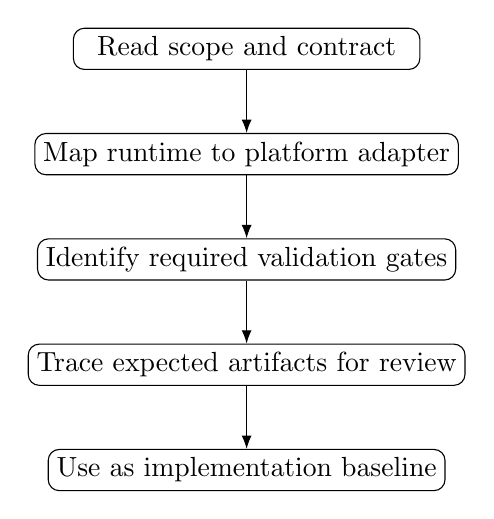
\begin{tikzpicture}[node distance=8mm and 12mm]
\node[box] (a) {Read scope and contract};
\node[box, below=of a] (b) {Map runtime to platform adapter};
\node[box, below=of b] (c) {Identify required validation gates};
\node[box, below=of c] (d) {Trace expected artifacts for review};
\node[box, below=of d] (e) {Use as implementation baseline};
\draw[line] (a) -- (b);
\draw[line] (b) -- (c);
\draw[line] (c) -- (d);
\draw[line] (d) -- (e);
\end{tikzpicture}
\caption{QEMU Deliverable 01: End-to-End Design Flow}
\end{figure}

\subsection*{Diagram B: Function Interaction and Attribute Flow}
\begin{figure}[H]
\centering
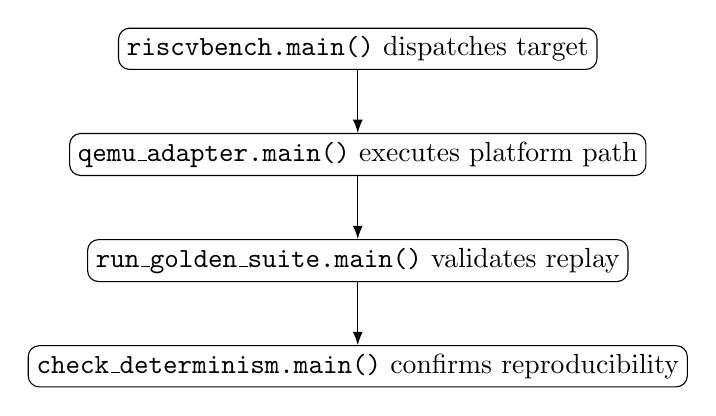
\begin{tikzpicture}[node distance=8mm and 12mm]
\node[box] (fa) {\texttt{riscvbench.main()} dispatches target};
\node[box, below=of fa] (fb) {\texttt{qemu\_adapter.main()} executes platform path};
\node[box, below=of fb] (fc) {\texttt{run\_golden\_suite.main()} validates replay};
\node[box, below=of fc] (fd) {\texttt{check\_determinism.main()} confirms reproducibility};
\draw[line] (fa) -- (fb);
\draw[line] (fb) -- (fc);
\draw[line] (fc) -- (fd);
\end{tikzpicture}
\caption{QEMU Deliverable 01: Function Interaction and Attribute Flow}
\end{figure}

\end{document}
